\section{Theoretical Foundations}
    \subsection{Aim}
        Within this experiment the working principle of a diode laser should be studied. In order to also get practical experience a diode laser is to be tuned to a wavelength of roughly \SI{780}{\nano\metre}
        to observe absorption of the laser light within a \ce{^{85}Rb}-, \ce{^{87}Rb}-vapor by doing a frequency scan. 
    
    \subsection{Working principle of general Lasers}
        The acronym Laser stands for \textit{light amplification by stimulated emission of radiation} and describes a light source, that emitts light of a fixed wavelength, which stays coherent over a long
        distances and is particulary suited for experiments due to its tunability. To achieve these properties a certain optical transition is stimulated and multiplied within an active medium.

        To start off an external \textbf{pump} excites electrons within an \textbf{active medium} from a lower energy state to a higher unoccupied energy state, from which these electrons will relax and the
        spontaneous emission of a photon will take place. During spontaneous emission photons are emitted isotropically into all directions but with the same energy, which corresponds to the energy difference
        between the higher and lower energy state $\Delta E = E_3 - E_2 = \frac{\text{hc}}{\lambda}$. The active medium is located in a \textbf{resonator}, which reflects the photons travelling along a certain axis and makes them pass trough the active medium
        multiple times. While doing this they can interact with the active medium in two more ways pictured in figure \ref{fig:prozesse}. They can be absorbed and excite an electron to a higher energy state or
        induce the stimulated emission of a second coherent photon in connection to an electron relaxing in the same way, as the electron, that spontaneously emitted an photon by relaxing. Due to the boundary conditions wihtin 
        the resonator modes will develop and increase their intensity, as the photons of the mode will induce stimulated emission of coherent photons, who will then also contribute to the mode. In order to always 
        have the possibility of stimulated emission a population inversion has to be created. This means that the electron density in the higher energy state is higher than in the lower enrergy state. To enable
        the possibility of inversion population one needs a system of at least three energy states. Given a system of four energy states the pump then excites electron from the ground state $E_{\text{1}}$ into 
        the highest energy state $E_{\text{4}}$. These excited electrons then relax into the second highest energy state $E_{\text{3}}$ by a high possibility $P_{\text{43}}$. From there they relax into the 
        second longest energy state $E_{\text{2}}$ by stimulated emission and afterwards into the ground state. To keep population inversion the transitions $4\rightarrow3$ and $2\rightarrow1$ have to be fast in
        comparison to the optical transition $3\rightarrow2$. This means the transition probabilities $P_{\text{43}}$ and $P_{\text{21}}$ have to be higher than $P_{\text{32}}$. Additionally the pump of 
        electrons from $E_{\text{1}}$ to $E_{\text{4}}$ needs to compensate for the amount of relaxing electrons.

        \begin{figure}[h]
            \centering
            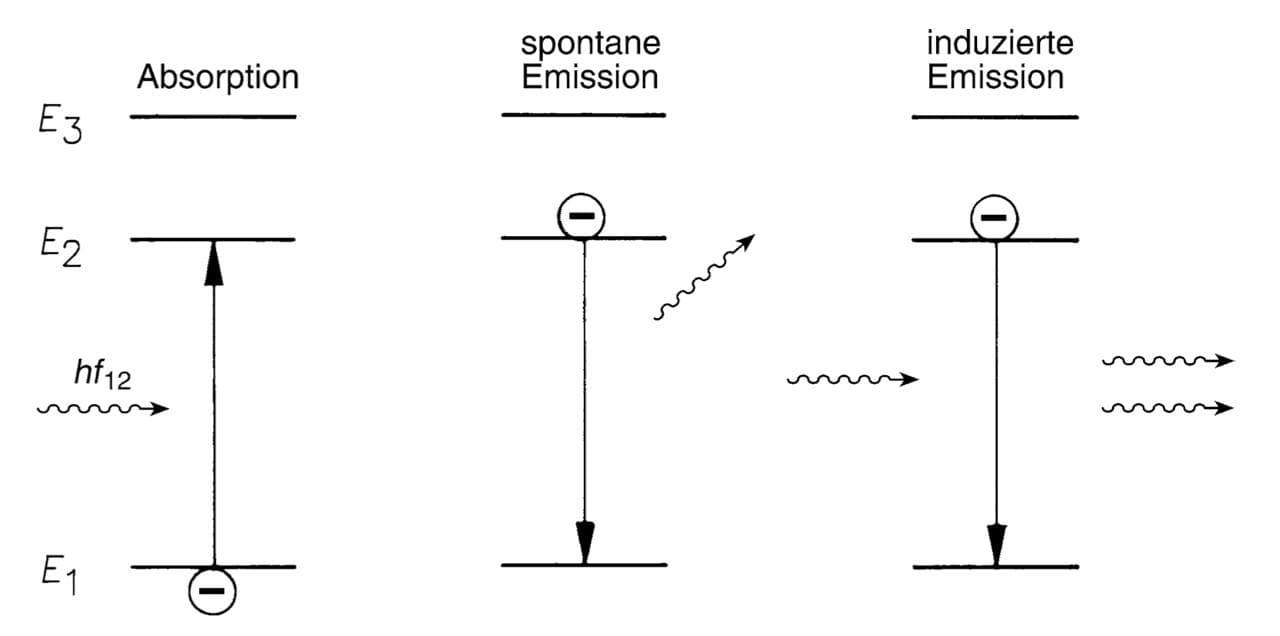
\includegraphics[width = 0.7\textwidth]{pictures/prozesse.jpg}
            \caption{Schemes of the possible light-matter-interactions of absorption, spontaneous and stimulated (induzierte) emission. $E_{1,2,3}$ mark different atomic energy levels, $h$ the planck contant and $f_{1,2}$ the photons frequency, which is propotional to $\Delta E_{12}$. Taken from \cite{eichler_laser_2015}.}
            \label{fig:prozesse}
        \end{figure}
        
        \FloatBarrier


    \subsection{Diode Lasers}
        \subsubsection{Working Principle}
            For diode lasers the same principles of a pump, stimulated emission within an active medium and population inversion can be applied. Additionaly some adaptions have to be done to correct for the solid 
            state properties of the active medium, as there are now longer well defined energy states in the form of atomic orbitals. Instead the nergy states now correspond to different energy bands wihtin the solid 
            states band structure. 
            Every solid state body has a valence band, which is the highest occupied band below the Fermi-Energy and a conduction band, which is the lowest unoccupied energy band above the Fermi-Energy. The energy
            difference between these two bands is called band gap $\Delta E = E_{\text{CB}} - E_{\text{VB}} = \frac{\text{hc}}{\lambda}$ and roughly defines the energy of a diode lasers light. 
            In this setup a pn-junction-diode is used as the active medium. A pn-junction constists of a highly n-doted layer, which is stacked onto a highly p-doted layer. A highly n-doted layer leeds to an 
            increase of the Fermi-Energy and the insertion of electrons into the conduction band. Vice versa a highly p-doted layer leeds to a lowered Fermi-Energy and the creation of holes in the valence band. 
            These processes are depicted in figure \ref{fig:pn_doted}.  

            \begin{figure}[h]
                \centering
                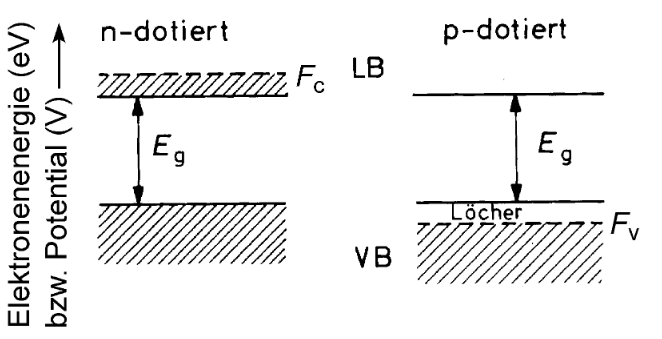
\includegraphics[width = 0.4\textwidth]{pictures/pn_doted.png}
                \caption{The increased Fermi-Energy within the conduction band for highly n-doted materials and the decreased Fermi-Energy within the valence band for highly p-doted materials, inserting electrons into the conduction band or creating holes in the valence band. Taken from \cite{eichler_laser_2015}.}
                \label{fig:pn_doted}
             \end{figure}
         
             \FloatBarrier
         
            When the two layers a brought together a pn-junction is formed, which only conducts a current into one direction, while it acts as an insulator for the other current direction. If a current is applied
            to the junction in the conduction direction, the holes will diffuse into the n-doted layer and the electrons into the p-doted layer. The creates the in figure \ref{fig:eh_diffusion} depicted active 
            area of the length $d$, in which a population inversion is created and the electron-hole pairs recombine, emitting photons of the band-gap energy isotropically.   
         
            \begin{figure}[h]
                \centering
                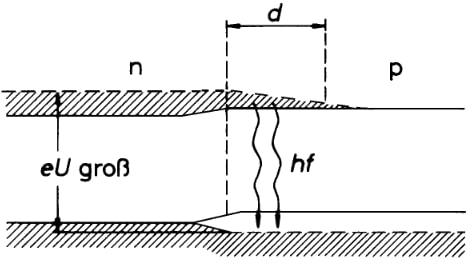
\includegraphics[width = 0.4\textwidth]{pictures/eh_diffusion.jpg}
                \caption{The diffusion of electrons and holes into the active layer by application of a current and the emission of photons by recombination of electron-hole-pairs. Taken from \cite{tu_dortmund_versuchsanleitung_2022-1}.}
                \label{fig:eh_diffusion}
            \end{figure}
        
            \FloatBarrier

            These spontaneously emitted photons are kept within the active layer as depicted in figure \ref{fig:diode_laser_scheme}, because the refractive index of the active layer is higher than the one of the 
            neighbouring layers and the light is thus totally reflected. The sides of the diode act as fully or partially reflecting mirrors creating an \textbf{internal resonator}, in which the reflected photons
            induce stimulated emission in the active layer and lay the foundation for lasing. The created light exits the diode on the partially reflecting side as a strongly diverging beam with a large bandwidth.  

             \begin{figure}[h]
                \centering
                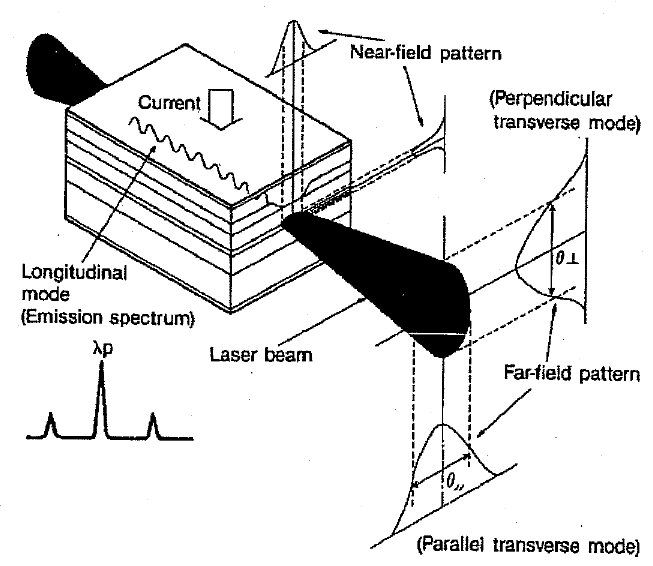
\includegraphics[width = 0.4\textwidth]{pictures/diode_laser_scheme.png}
                \caption{The diffusion of electrons and holes into the active layer by application of a current and the emission of photons by recombination of electron-hole-pairs. Taken from \cite{tu_dortmund_versuchsanleitung_2022-1}.}
                \label{fig:diode_laser_scheme}
             \end{figure}
         
             \FloatBarrier

            These two deficits are compensated for by the in figure \ref{fig:littrow} optical setup, that remains the laser in a so called \textit{Littrow}-configuration and creates an additional 
            \textbf{external resonator}. The setup constists of lense, which collimates the light exiting the laser diode and a grating, at which the collimated beam is diffracted. This happens in a way, that
            the zero-order-maximum, i.e. the reflected beam, is guided out of the laser setup as the operating beam, while the first-order-maximum is diffracted back into the laser diode. Thus the new 
            external resonator is formed between the grating and the fully reflective backend of the laser diode. The wavelength of
            the light diffracted back into the laser diode, has to fulfill the condition for the first-order-maximum at the given angle of the grating. The back-reflected beam helps selecting a certain
            wavelength in a way, that is further discussed in the section on the gain curves of a diode laser.   


            \begin{figure}[h]
                \centering
                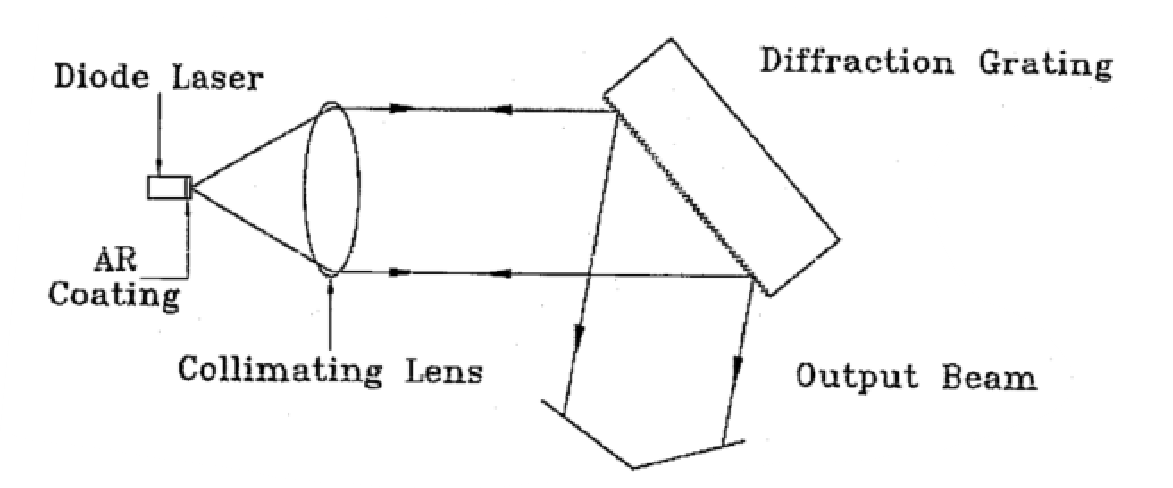
\includegraphics[width = 0.6\textwidth]{pictures/littrow.png}
                \caption{The diffusion of electrons and holes into the active layer by application of a current and the emission of photons by recombination of electron-hole-pairs. Taken from \cite{tu_dortmund_versuchsanleitung_2022-1}.}
                \label{fig:littrow}
            \end{figure}
        
            \FloatBarrier


        \subsubsection{Gain Curves}
            To emitt light of a well defined frequency the laser has to lase in fixed combination of a mode of the internal and one of the external resonator. Which modes will be selected, is determined by
            the gain curves depicted in figure \ref{fig:gain_curves}. They show the different gains of laser intensity via different contributions against the laser wavelength. The wavelength for which the
            total amount of gain by all contributing factors, namely \textbf{Medium}, \textbf{Internal Cavity}, \textbf{Grating Feedback} and \textbf{External Cavity}, is the highest will be the lasing 
            frequency and the closest internal and external modes will be the lasing modes.\newline

            \begin{figure}[h]
                \centering
                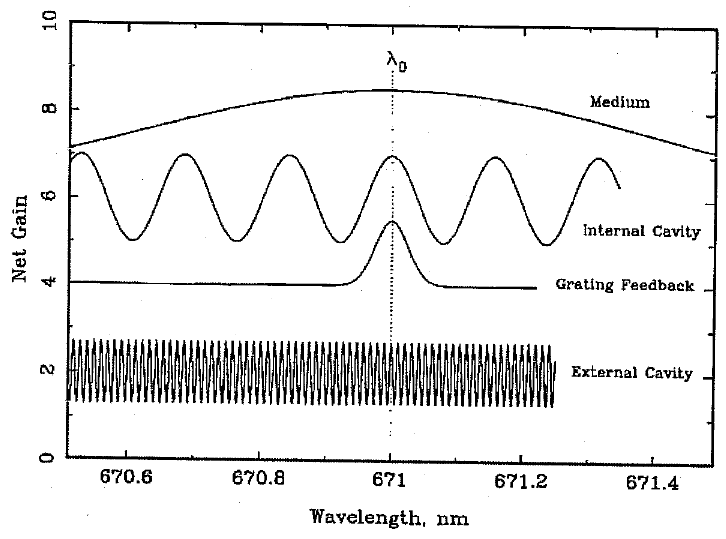
\includegraphics[width = 0.6\textwidth]{pictures/gain_curves.png}
                \caption{The contributing gain curves for the diode laser used in the setup. Taken from \cite{tu_dortmund_versuchsanleitung_2022-1}.}
                \label{fig:gain_curves}
            \end{figure}
        
            \FloatBarrier

            %\newline
            The \textbf{Medium-Gain} has a widespread peak with its maximum at the wavelength corresponding to the energy gap of the active medium. Thus the choice of the medium is the main factor governing
            the lasers wavelength. The position of the peak has a small dependence on the laser diodes temperatur, which is neglectible for the given experiment.\newline 

            %\newline
            The gain of the \textbf{Internal Cavity} oscillates and has it peaks at the wavelengths of the longitudinal modes, which develop in the internal cavity. The distance between the different peaks is 
            inversely propotional to the length of the resonator, i.e. the length of the diode, and thus rather large.\newline

            %\newline
            The gain of the \textbf{Grating Feedback} has a sole peak at the frequency of the first-order refracted light, that is reflected back into the diode and can thus be changed by varying the angle of 
            the grating.\newline
            
            %\newline
            The gain of the \textbf{External Cavity} oscillates equivalently to the gain of the internal cavity but has a way smaller distance between the mode peaks, as the external resonator is way longer in
            comparison to the internal resonator. The position of the modes can be varied by changing the position of the grating and consequently the length of the external cavity. 
    
    

    \subsection{Rubidium}
        The $\text{5S}_{\frac{1}{2}}$-electrons of the Rubidium isotopes \ce{^{85}Rb} and \ce{^{87}Rb} can be excited into the $\text{5P}_{\frac{3}{2}}$-orbitals with photons of a wavelength of roughly 
        \SI{780}{\nano\metre}. A closer look at the in figure \ref{fig:Rb} depicted fine-structure of the two isotopes shows two charateristic transitions per isotope. If you transmit a beam trough Rubidium-vapor
        and sligthly vary the beam wavelength around \SI{780}{\nano\metre}, one will detect four dips in the transmitted intensity. Each dip is located at the wavelength equivalent to the 
        excitation energy of the particular transition.  
        
        
        \begin{figure}[h]
            \centering
            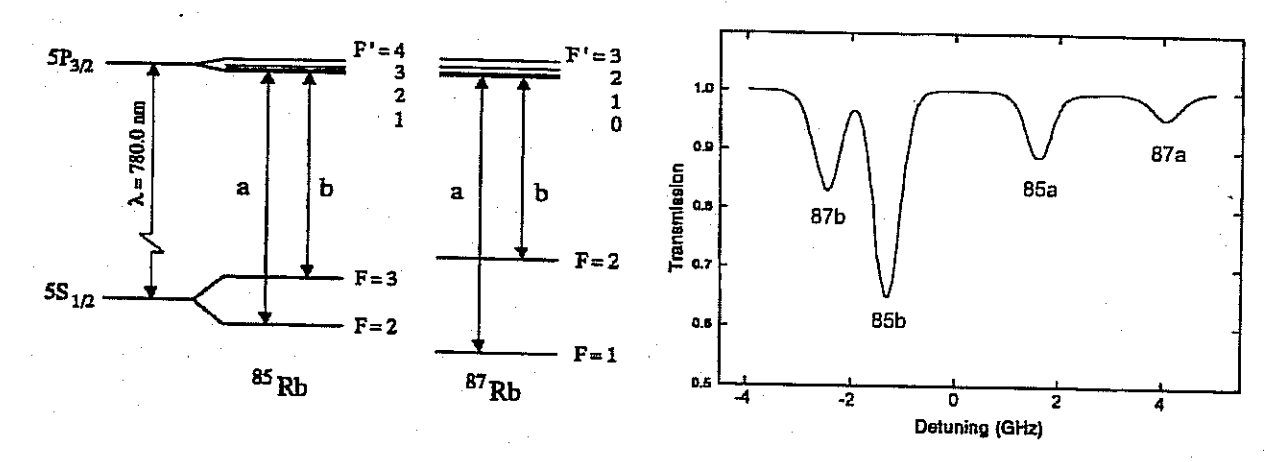
\includegraphics[width = 0.6\textwidth]{pictures/Rb.png}
            \caption{The four possible transitions from the $\text{5S}_{\frac{1}{2}}$-orbital to the $\text{5P}_{\frac{3}{2}}$-orbital for the two Rubidium isotopes and the corresponding dips in a transmission measurement. Taken from \cite{tu_dortmund_versuchsanleitung_2022-1}.}
            \label{fig:Rb}
        \end{figure}
    
        \FloatBarrier
         
        